\subsection{Subjects}
For the experiment 12 able-bodied subjects were recruited (10 male, 2 female - 11 right-handed, 1 left-handed) by contacting fellow undergraduate biomedical engineering students at Aalborg University. All subjects participated in the entire experiment, and was initially informed of the research aim, and instructed about the procedures during the experiment. Entire data sets from three subjects was excluded. The cause for exclusion for one subject was due to data that did not correspond with the instructed movements, and the remaining two was due to baseline data being similar in amplitude compared to EMG amplitude of high contraction movements. All subjects participated voluntarily, and did not receive any monetary reimbursement. 

\subsection{Data acquisition}
EMG signals and inertial information were recorded with the Myo armband from Thalmic Labs - a 8 channel dry electrode armband with a 200 Hz EMG sampling rate and 50 Hz IMU sampling rate. The Myo armband has been suggested as a suitable data acquisition system for pattern classification \cite{Mendez2017}, but not yet for a regression-based control scheme. 
The armband was placed around the thickest part of the dominant forearm, approximately 1/4 of the length towards the wrist distal of the elbow. For a close contact between the forearm and armband, clips was used to tighten the fit if necessary. All data acquisition, processing, data analysis and testing was performed in MATLAB and MATLAB's Graphical User Interface Development Environment.

In the training data acquisition the subjects were instructed to perform four different wrist movements of 2 DOF's depicted in figure \ref{fig:wristmovement} in three different limb positions depicted in figure \ref{fig:limbpositions}. Each movement was performed with four different EMG intensities of the Maximum Voluntary Contraction (MVC) in each limb position (baseline, 30 \%, 50 \% and 80 \%). To ensure that correct fractions of the EMG intensity were recorded, a Graphical User Interface (GUI) was build to provide real-time feedback for the subject. Initially the MVC was recorded, scaled to 1 and set as reference point for the following trials. A trapeze was drawn for each data acquisition trial, where the plateau depicted the desired fraction of the MVC. A cursor visualized the EMG signal, and moved continuously with time. The vertical position of the cursor was calculated as the mean of the absolute EMG signal across all channels in a 200 ms window, and scaled according to the MVC. The subject adjusted the height of the cursor by varying the contraction intensity, and was instructed to follow the trapeze as precise as possible. Especially in the plateau phase since only the steady state EMG was used for data analysis. \textbf{Justify that steady state is sufficient to use for control.} The duration of each data acquisition trial was 10 s, where the plateau phase was 3 s. To avoid fatigue the subjects had a 10 s break between trials of different intensities. Between limb positions subjects were given a 5 min rest. Accelerometer data was additionally recorded in each trial. All trials were performed while standing.
Additional 50 \% of MVC EMG data was acquired for each wrist movement in all limb positions for offline testing.

The recorded EMG data was filtered using a $2^{nd}$ order Butterworth high-pass filter with a 10 Hz cut-off to remove movement artefacts. 

\begin{figure}[thpb]
	\centering
	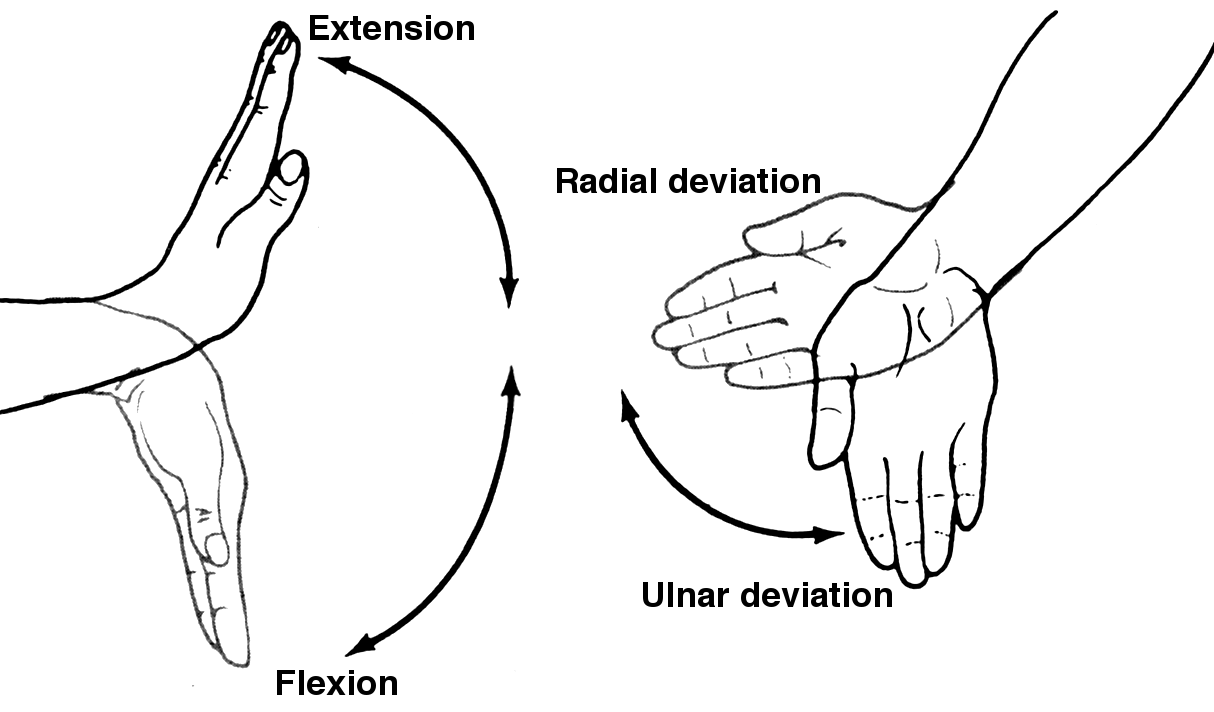
\includegraphics[width=0.4\textwidth]{Figures/wristmovement}  %<--but is not needed.
	\caption{Illustration of the two DOF's performed (P1: flexion, P2: extension and P3: radial deviation, P4: ulnar deviation)}
	\label{fig:wristmovement}  %<--give the figure a label, so you can reference!
\end{figure}

\begin{figure}[thpb]
	\centering
	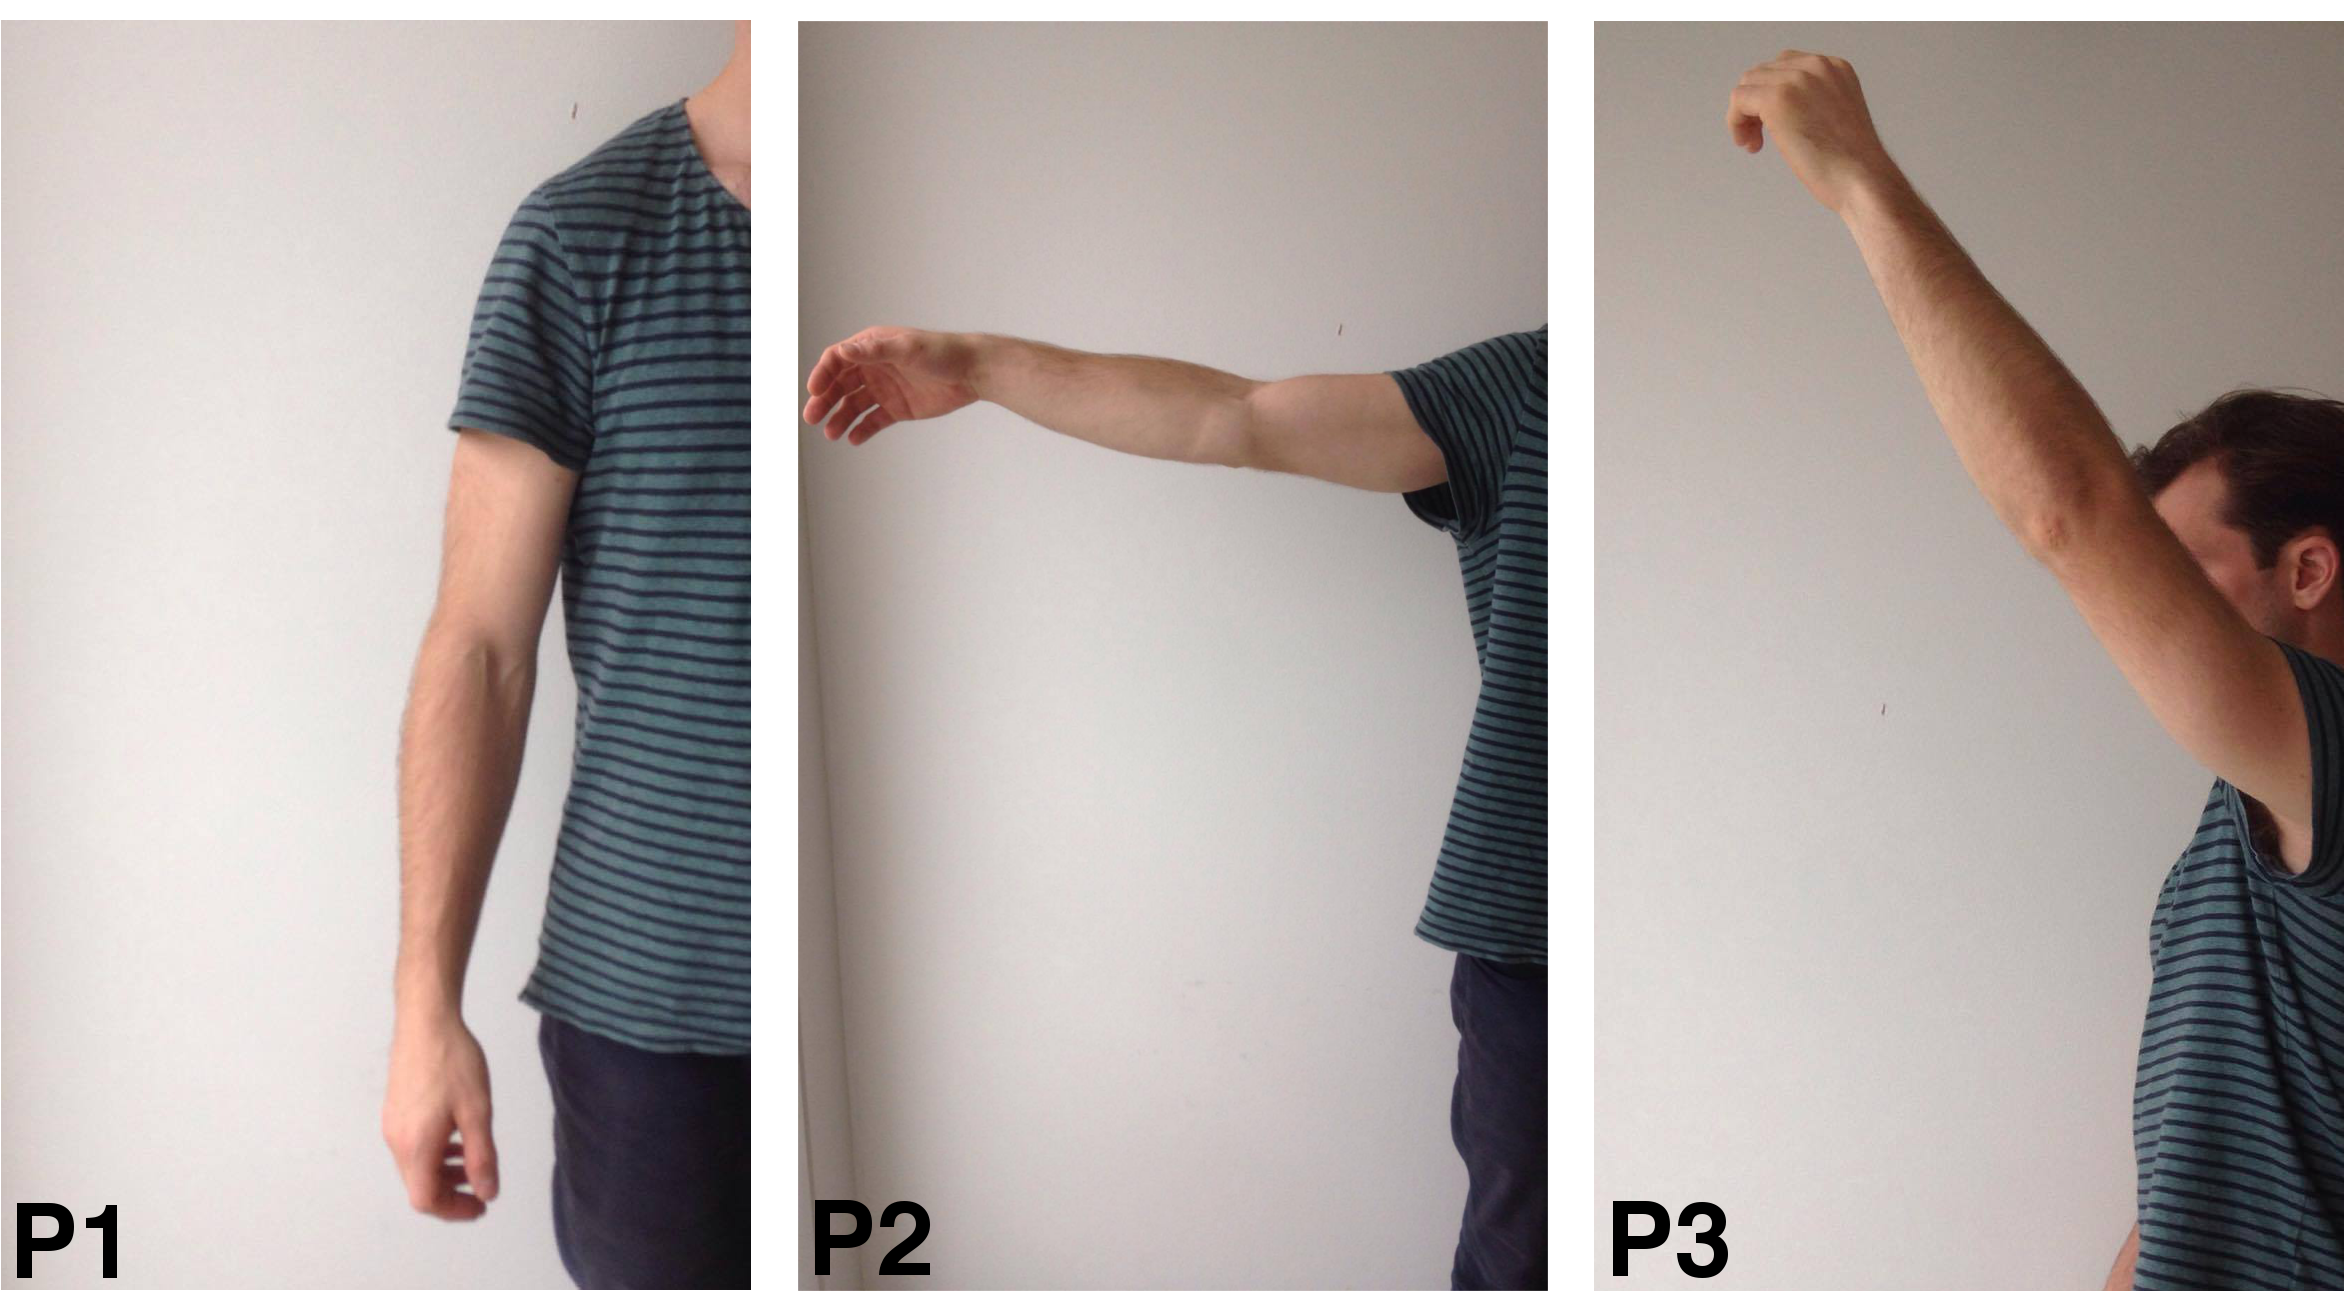
\includegraphics[width=0.4\textwidth]{Figures/limb_pos}  %<--but is not needed.
	\caption{Illustration of the limb positions performed. P1: relaxed along the torso, P2: 90 degrees horizontally of the torso and P3: 135 degrees vertically of the torso}
	\label{fig:limbpositions}  %<--give the figure a label, so you can reference!
\end{figure}

\subsection{Feature extraction}
Features were extracted in a 200 ms window with a 50 \% overlap, which is an acceptable segmentation for preserving information of the signal in static contractions \cite{Farfan2010}.
In a previous study \cite{hahne2014} it was shown that logarithmizing the variance of EMG the variance linearises, and has yielded robust control of wrist movements in a relaxed limb position when used in linear regression. The Logarithmic Variance (LogVar) was therefore extracted as a feature, and was calculated as given by equation \ref{eq:logvar}:

\begin{equation} \label{eq:logvar}
log(\sigma^2) = log(\frac{\sum\limits_{i=1}^N(x_i - \mu)^2}{N})
\end{equation}
where N expresses the length of the window, $x_i$ is the $i^th$ sample of the signal and $\mu$ is the mean. 

The commonly used Mean Absolute Value (MAV) feature was additionally extracted, and calculated as given by equation \ref{eq:mav}:

\begin{equation} \label{eq:mav}
MAV = \frac{1}{N}\sum\limits_{i=1}^N|x_i|
\end{equation}
where N is the length of the window, and $x_i$ is the signal of $i$ samples.

MAV is directly correlated with change in EMG amplitude. No study has examined whether MAV contains linear properties, but EMG signals has heteroscedastic properties \cite{rasool2012} and the MAV feature might therefore not contain direct linear properties.

The Mean Value (MV) was extracted from the accelerometer data, similarly to a previous study \cite{Krasoulis2015} testing the effect of limb position using classification as control scheme. 

The extracted EMG features for the individual wrist movements were examined through a Principal Component Analysis, to evaluate, whether the different movements were distinguishable or new training data should be acquired.

\subsection{Regression model}
One regressor was trained for each wrist movement for both features; four regressors trained for each feature, and four for each feature where accelerometer data was included. Each regressor was trained based on multivariate linear regression and calculated as given by equation \ref{eq:linearregression}:

\begin{equation} \label{eq:linearregression}
\hat{Y} = \alpha + \beta_1 X_{1} + \beta_2 X_{2} + ... + \beta_i X_{i}
\end{equation}
where $\hat{Y}$ is the estimated value, $X_i$ are the predictors, $\beta_i$ are the regression coefficients in the sampled population, and $\alpha$ is the predicted value of $Y$ at $X_{i} = 0$. $\beta_i$ and $\alpha$ are fitted for each regressor using the extracted feature data for each channel in $X_i$. The mean of the absolute values of the actual EMG across all channels scaled in relation to the MVC is set as the $\hat{Y}$. The features for all wrist movements are included as $X_i$ in the training of each regressor. However, only the desired wrist movement the regressor is fitted for, is trained with the actual estimated values. The remaining predictors are given 0 as estimated values. This procedure was applied for the regressors to more precisely recognize the performed movement. The features for all intensities in all limb positions were used in the training of the regressors.

\subsection{Offline testing}
The accuracy of the regressors was examined both qualitatively and quantitatively when using both training and test data. A qualitative test was performed by superimposing the regressor output on the actual data. The superimposition illustrated whether the right regressor reacted on the performed movement, and how accurate it responded compared to the actual data. For the quantitative analysis the Root Mean Square Error(RMSE) was calculated to compare through statistical analysis, which feature had the lowest error, and whether the regressors were overfitted when tested with new input data. Furthermore, the accuracy of the regressors trained with inclusion of accelerometer data was compared to the regressors trained only using EMG feature data. The RMSE was calculated as given by equation \ref{eq:rmse}:

\begin{equation}\label{eq:rmse}
RMSE = \sqrt{\frac{\sum\limits_{i=1}^N(y_i - \hat{y_i})^2}{N}}
\end{equation}
where N is the length of the window, $y_i$ is the $i^{th}$ variable of the actual data and $\hat{y_i}$ is the $i^{th}$ output of the regressor.

It was decided, which statistical analysis to apply, through a Kolmogorov-Smirnov test that assesses whether the data populations were normal distributed. An ANOVA test was applied if the data population belonged to a normal distribution, if not a Friedman's test was applied, which is the non-parametric correspondent to an ANOVA test.

\subsection{Online testing}
To investigate the effect of limb position in the regression control scheme an online virtual environment was developed, depicted in figure \ref{fig:tagets}

	\begin{figure}[thpb]
		\centering
		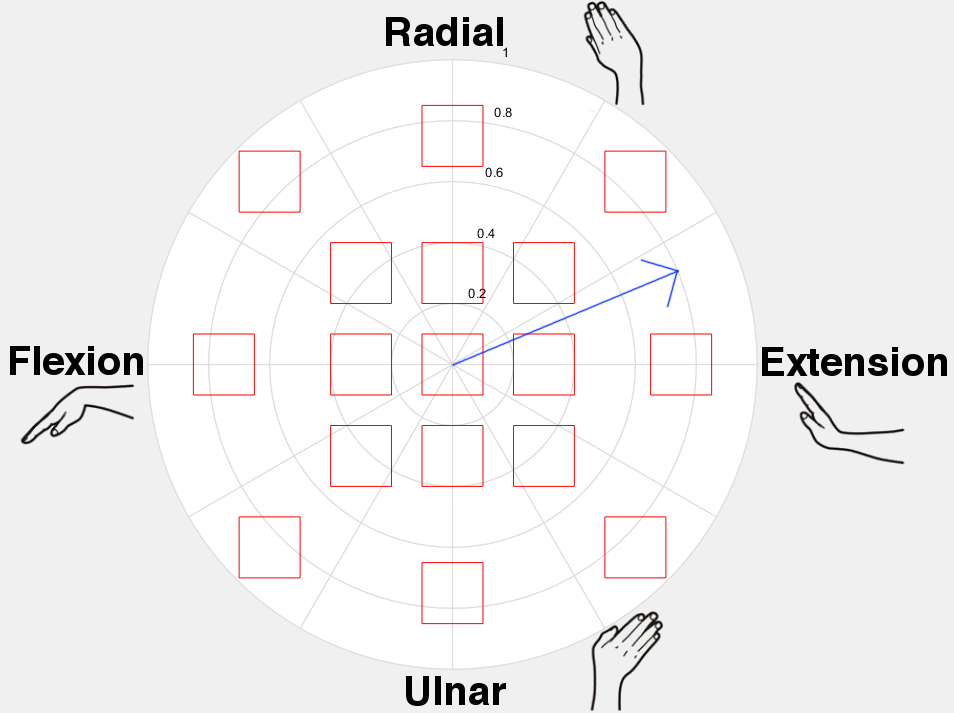
\includegraphics[scale=0.25]{Figures/Target}
		\caption{A vector originated from origo depicted the EMG signal, where the length of the vector represented the EMG intensity, and direction was based on the movement performed. The wrist flexion-extension was mapped to the x-axis, and the radial-ulnar deviation was mapped to y-axis. The vector returned to the target located around origo when no contraction was made. For the subject to reach the targets in the diagonals, a simultaneous movement must be performed. One target was shown at a time. When a target was reached, the vector had to return to the centred target for a new to appear. This gave the subject the same starting point when reaching each outer target. The procedure was performed until all targets had appeared. If a target was not reached within 30 s, it would disappear, and the vector had to return to the centred target.}
		\label{fig:targets}
	\end{figure}

 The time to complete a target-reaching task of sixteen targets was measured. 12 tests were performed by each subject; one in each limb position for each feature for the regressors trained with and without included accelerometer data. The performance score was calculated as the mean of time per reached target. Time to reach the centred target was not included in the performance score. Performance scores of the online test was compared between the different limb positions of the same feature, between all limb positions of the two features and between performance score obtained when using regressors trained with and without inclusion of accelerometer data. The same comparison was additionally applied for the amount of targets reached. The statistical analysis applied was again based on whether the populations were normal distributed or not.
%\subsection{Experimental Setup}
%EMG data was collected from ten able-bodied subjects. The subjects performed four different hand gestures. This study is only focus on two DOF, which are, flexion, extension, radial and ulnar deviation of the wrist. The order in the execution of the movements was the same for each subject. EMG signals were recorded with Myo armband, positioned in the forearm of the dominant hand of the subjects. Myo armband counts with eight medical grade stainless steel surface EMG sensors, with a sampling rate of 200Hz. It counts with nine axis IMU which provides information about position and orientation of the arm combining three axis accelerometer, three axis gyroscope and three axis magnetometer. %It is capable of pulling EMG data at a sample rate of 200 Hz. 
%%Furthermore its nine axis IMU provides information about position and orientation of the arm combining three axis accelerometer, three axis gyroscope and three axis magnetometer.\\   
%The procedure was performed in three different limb positions. In order to avoid shoulder fatigue a relaxation period was given between trials. The subjects were instructed to keep the fingers in repose. %move the fingers during the data acquisition. 
%The process was performed in a standing position. \\ %figure hand and limb positions
% 
% In order to acquire the training data necessary to build the regressor, a graphical user interface (GUI) was implemented in MATLAB. %Firstly baseline was meassure holding the forearm relaxed and the wrist in a neutral position for the corresponding limb position. This measure was substracted from the signal afterwards to be able to remove the present artefacts. Subsequently maximum voluntary contraction (MVC) was meassure. The MVC  was calculated as a mean of the maximum values in each of the eight cannels, and was set as a normalized reference point of 1.
% The data acquisition was depicted through a trapeze. %MVC was set as the desired value before data acquisition. Consequently each hand gesture was performed as a fraction of the MVC. 
% At the begining of the training data collection two second resting phase was given followed by two seconds ascending slope to reach the plateau phase, with a duration of three seconds. Afterwards a descending phase of two seconds and a resting phase of one second finalized the data acquisition. The total acquisition time was ten seconds per hand movement.
%
%	%\subsection{Maintaining the Integrity of the Specifications}
%	
%	%The template is used to format your paper and style the text. All margins, column widths, line spaces, and text fonts are prescribed; please do not alter them. You may note peculiarities. For example, the head margin in this template measures proportionately more than is customary. This measurement and others are deliberate, using specifications that anticipate your paper as one part of the entire proceedings, and not as an independent document. Please do not revise any of the current designations
%	%	\begin{figure}[thpb]
%	%	\centering
%		%\framebox{\parbox{3in}{We suggest that you use a text box to insert a graphic (which is ideally a 300 dpi TIFF or EPS file, with all fonts embedded) because, in an document, this method is somewhat more stable than directly inserting a picture.
%	
%	%	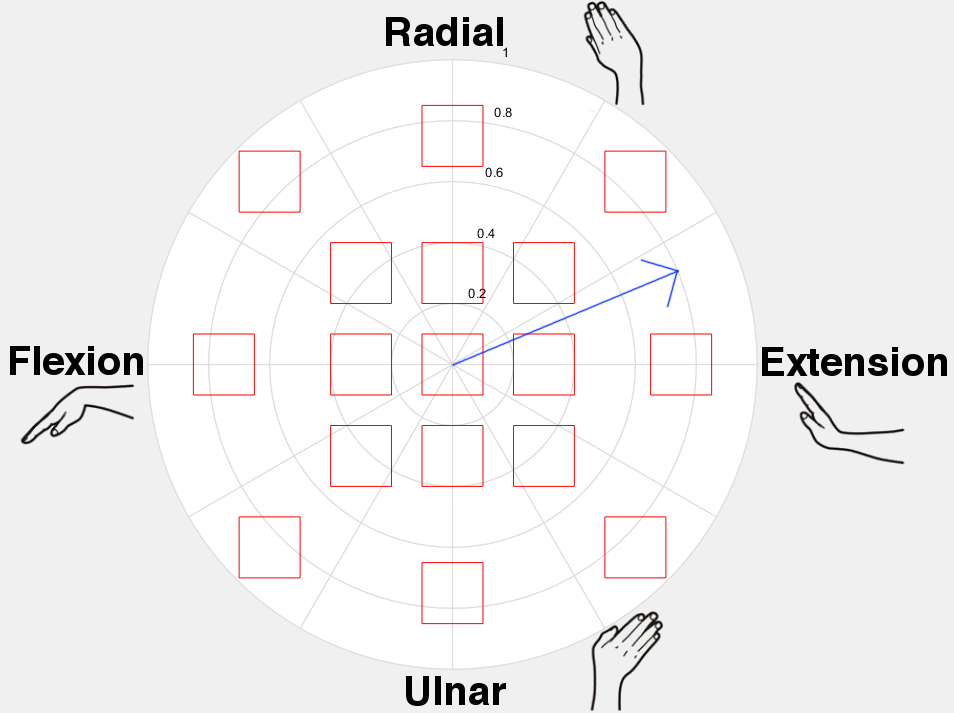
\includegraphics[scale=0.25]{Figures/Target}
%	%	\caption{Something}
%	%	\label{figurelabel}
%	%\end{figure}
%\begin{figure}[htb]
%	\centering
%	\subfigure[]{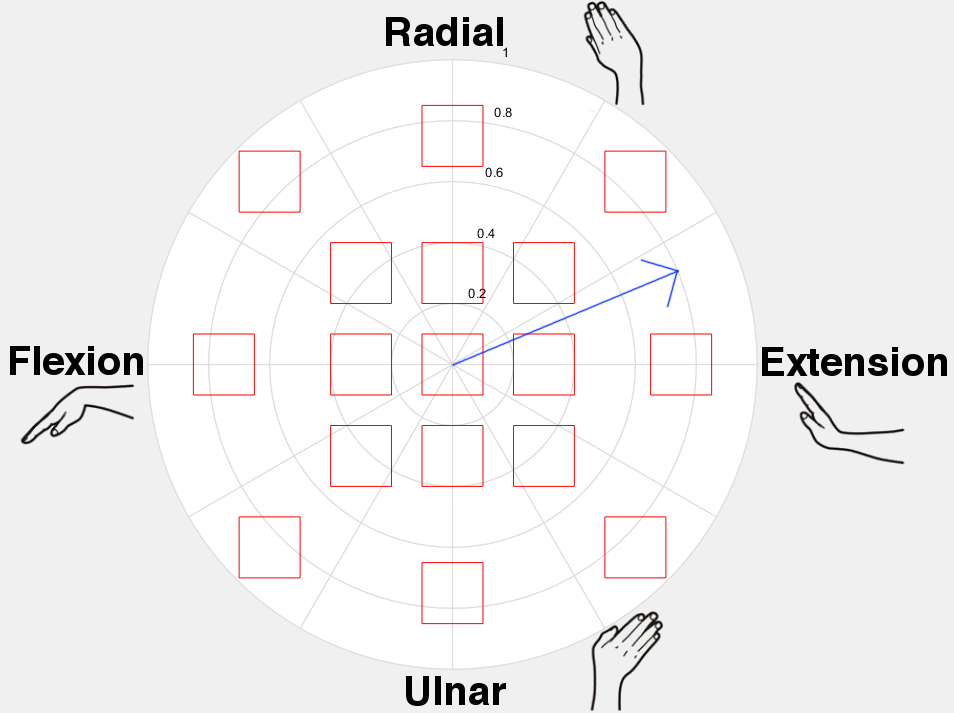
\includegraphics[width=70mm]{Figures/Target}}
%	\subfigure[]{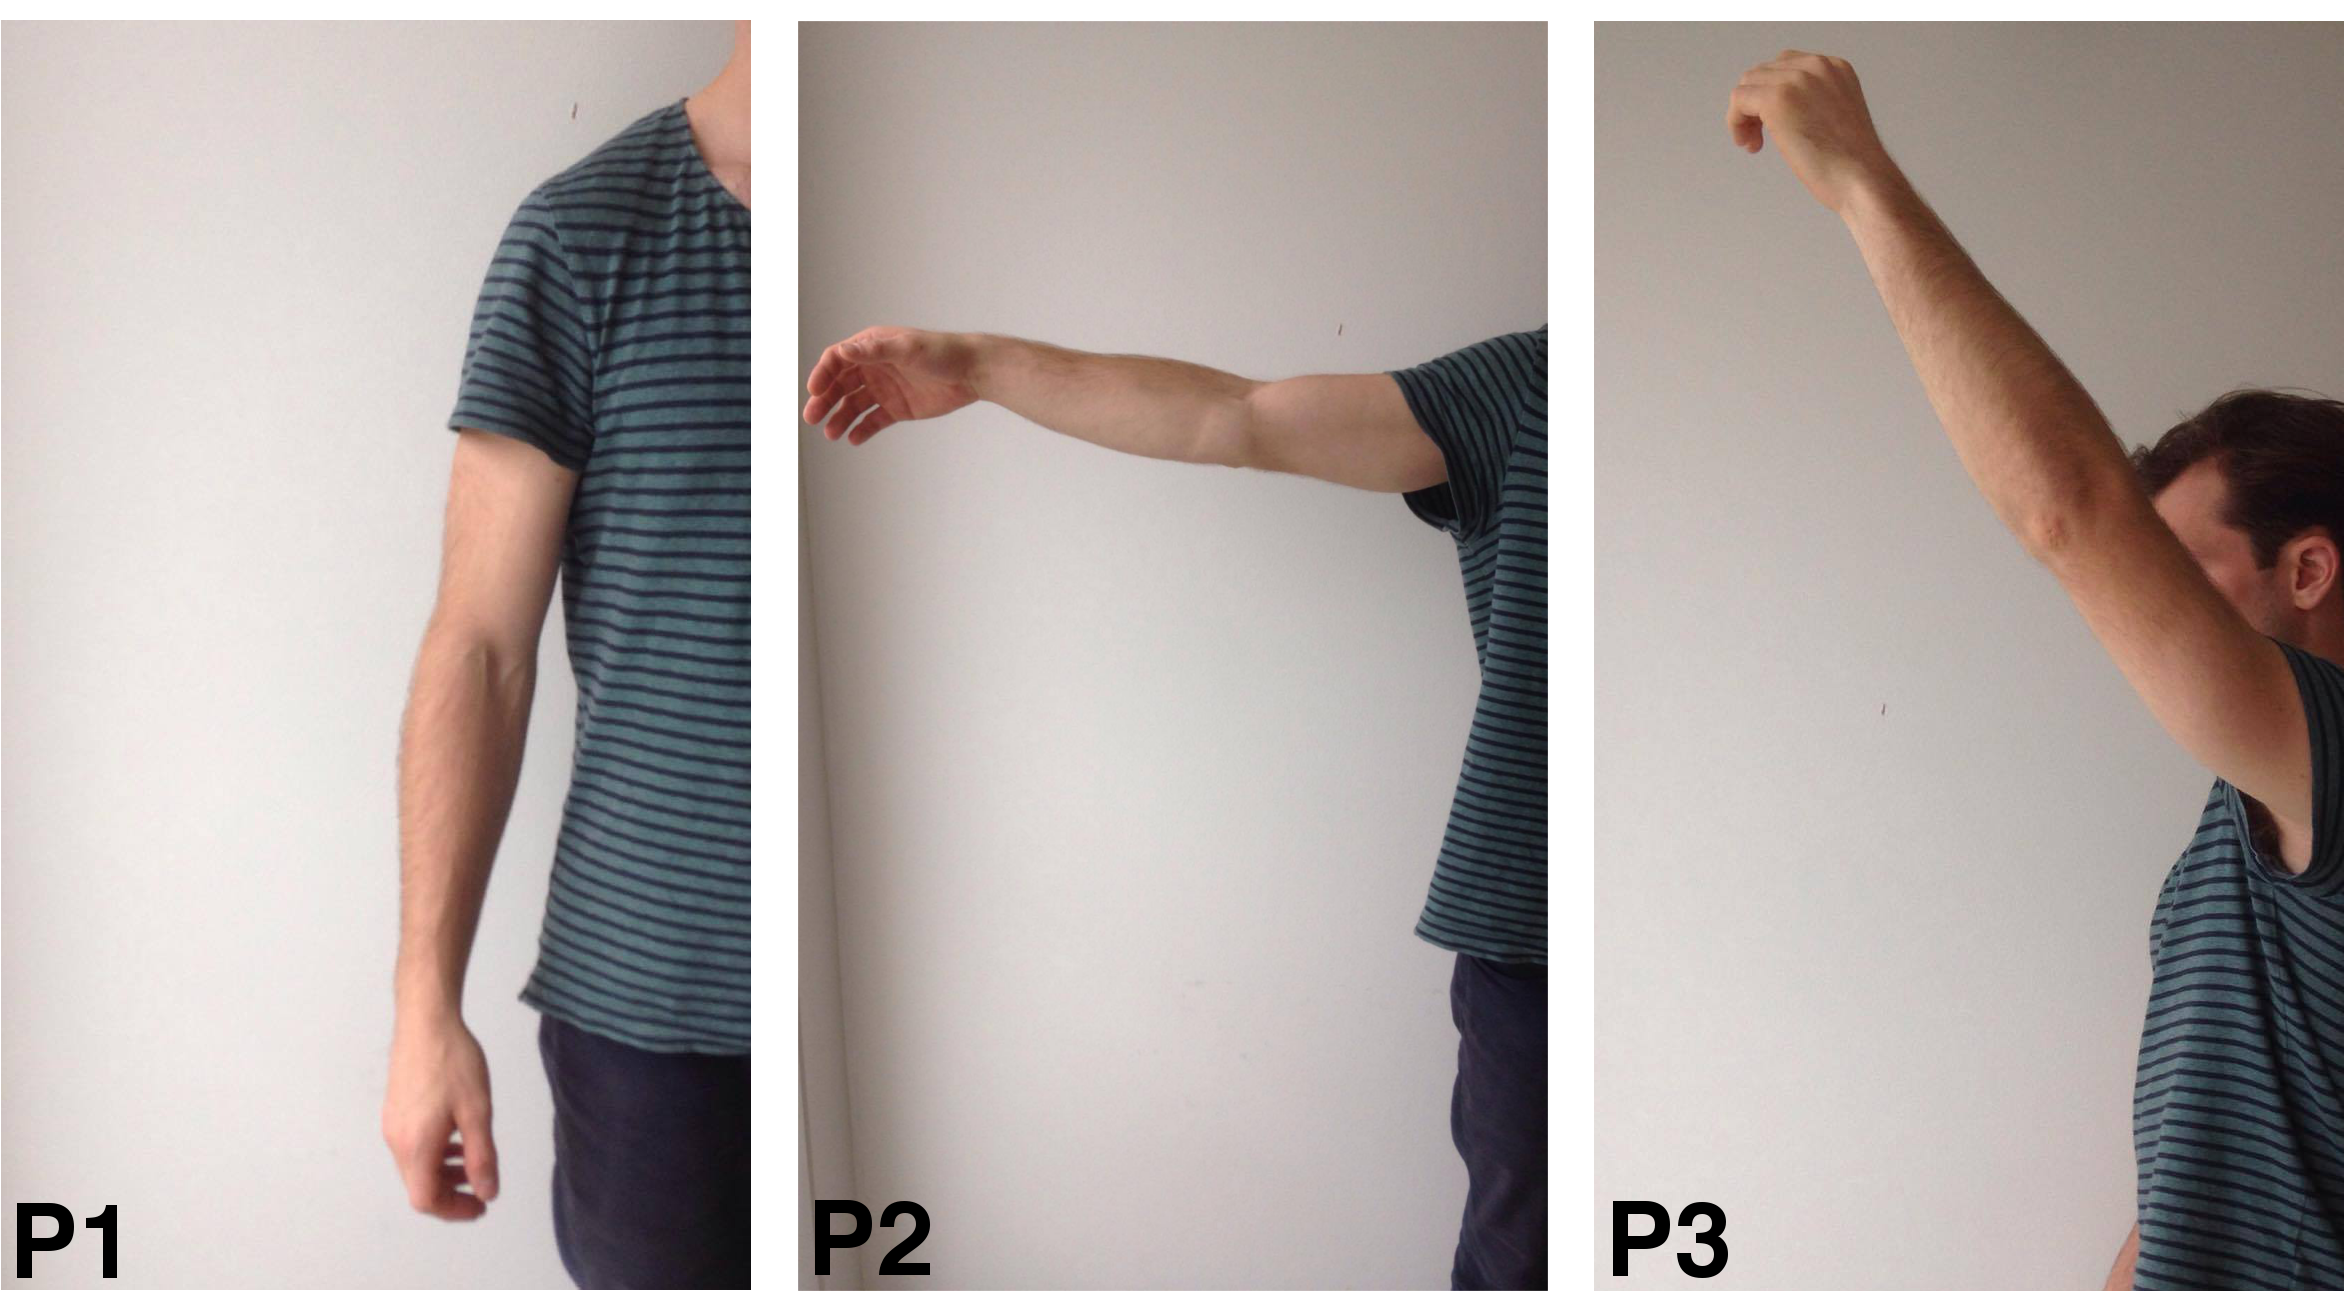
\includegraphics[width=70mm]{Figures/limb_pos}}
%	%\subfigure[Lannisters]{\includegraphics[width=80mm]{./lannisters}}
%	\caption{Experimental Setup: (a) Something blabla (b) Different limb positions performed during the study} \label{fig:setup}
%\end{figure}%Finish caption
%	\subsection{Preprocessing}
%	For this study the EMG data acquired were filtered using a second-order Butterworth high-pass filter, cutoff frequency ($f_c$=10Hz), to avoid low frequency movement artefacts in the recorded signal.\\
%	%review two states part trapeze!!
%	%The EMG signal is the result of the addition of different motor unit action potential trains (MUAPTs). Through the data acquisition phase EMG signal can be divided into two main states. The transient state, related with the beginning phase of the muscle contraction and the steady state which is the stable phase of the muscle contraction when a constant position is held \cite{mobarak2014}. Although the steady state only contains a short temporal structure of the patterns involved in the contraction of the muscle \cite{mobarakm2014}, studies has shown that it is possible to achieve online continuous control using steady state EMG signals.This could be due to the fact that a larger amount of meaningful data is contained in this muscle contraction phase \cite{mobarakm2014}. For the training of the control system in this project the steady signal was then used.
%	
%	\subsection{Feature extraction}
%	The features were extracted creating a sliding-window of 40 samples with an overlapping of the 50\%. 
%	Two different time domain features were extracted, MAV as well as LogVar. MAV represent the amplitud of the signal. It is defined as the average of the absolute values of the EMG signal and expresed as:
%	\begin{equation}
%	MAV = \frac{1}{N}\sum\limits_{i=1}^N|x_i|
%	\end{equation}
%	where N is the length of the signal, and $x_i$ is the signal of $i$ samples.
%	The LogVar is a nonlinear transformation of the variance, which has been shown linear properties compare to other time domain features. \cite{hanhe2014}
%	\begin{equation} \label{eq:logvar}
%	log(\sigma^2) = log(\frac{\sum\limits_{i=1}^N(x_i - \mu)^2}{N})
%	\end{equation}
%	where N expresses the length of the signal, $x_i$ is the $i^th$ sample of the signal and $\mu$ is the mean.
%	\subsection{Separability of data}
%Principal Component Analysis (PCA) was applied to be able to evaluate the quality of the features extracted from the EMG signals.
%	%This analysis tool express a set of correlated variables into non-correlated components. In that way, the data set can be expressed in a reduced dimensionality hyperspace using less but most representative variables which are the principal components. Through PCA is  possible to see significant outliers or if the clusters formed by the features can be easily distinguishable. This was done to avoid inaccurate training of the regressors. PCA was performed for each movement in each limb position. %and represented in three dimensional space.figure? 
%	\subsection{Data exclusion}
%	One of the subjects was not able to perform through the study properly. In order to ensure constant data those subjects were exclude.
%	(review this)
%	\subsection{Regression models}
%	The acquired data was used to built the different regressors that had been implemented, one for each movement under study and for both features. Multivariate linear regression as an extension of simple linear regression had been applied as is shown in \ref{reg}:
%\begin{equation}
%	\hat{Y} = \alpha + \beta_1 X_{1} + \beta_2 X_{2} + ... + \beta_i X_{i} + \epsilon_i
%		\label{reg}
%\end{equation}
%	where $Y$ is the dependent variable, $X_i$ are the independent variables, $\beta_i$ is the regression coefficient in the sampled population, $\alpha$ is the predicted value of $Y$ at $X = 0$ and $\epsilon$ is the error.
%	
%	\subsection{Regressor accuracy}
%	Superimposition\\
%	In order to examine the performance of the regressors the estimations of the regressor and the actual data for the two different features extracted had been superimposed. Thereby the behave of the regressor can be shown at different intensities and movements. Consequently whether other regression methods should be considered to obtain a lower error.\\
%	RMSE\\
%	To meassure the accuracy of the regressor, Root Mean Squared Error (RMSE) was calculated. RMSE is a calculation of the standard deviation of the residuals, that is, the difference between the estimated and the actual values.
%	%equation
%	\begin{equation}
%	RMSE = \sqrt{\frac{\sum\limits_{i=1}^N(y_i - \hat{y_i})^2}{N}}
%	\end{equation}
%	Where N is the length of the signal, $y_i$ is the $i^th$ variable of the actual data and $\hat{y_i}$ is the $i^th$ output of the regressor. The RMSE will be done for the regressor of each movement.\\
%	
	%Fitts Law\\
	%A modified version of Fitts' Law had been used to quantify the performance of the trained regressors. Fitts' Law describes that, the time it takes to do a rapid movement to reach a target area, is dependent on the distance to the target area, and the size of the target area. The law demonstrates that the information of any human motor tasks, is finite and only limited by the capabilities of the control system. The control exhibit a negative correlation between speed and accuracy. \cite{Kamavuako2014}
	%Fitts' Law calculates an \textit{Index of Difficulty} (ID) by \ref{eq:Fitts}
	
%	\begin{equation} \label{eq:Fitts}
	%ID = log_{2} \cdot (\frac{2D}{W})
	%\end{equation}
	
	%where D is distance to the targets and W is width of target area. The system in this study does not provide a reasonable scale for distance and target width, for this reason Fitts' Law cannot be apply as usual. Instead, the time it takes a subject to reach the targets as well as the number of targets reached will be noted to calculate a performance score as shown in \ref{eq:ourScore}.
	
	%\begin{equation} \label{eq:ourScore}
	%Score = \frac{time}{targets\ reached}
	%\end{equation}
	%Consequently low score results represent the best performance.
	%To accomplish the modified Fitts' Law test a compass-plot was implemented in the GUI Fig.\ref{figurelabel}. The subjects had to reach 16 targets distributed around the origin in two different radius. This allows to test the proportional control. The targets were fixed in the diagonals of the compass-plot to be able to test simultaneous control. The amount of targets reached in each quadrant gives important information about the regressor performance as well as, providing the weak directions.
	
	
	
